\documentclass[t,serif]{beamer}
\usepackage[portuguese,brazil]{babel} % nomes em portugues
\usepackage[utf8]{inputenc} % acentuacao
\usepackage[T1]{fontenc}
\usepackage{ae} % separacao de sílabas de palavras com acento
\usepackage{icomma}         % acerta espacamento quando a vi­rgula
\usepackage{color}
\usepackage{enumerate}
\usepackage{courier}

\usetheme{Boadilla}
% \usetheme{Copenhagen}
%\usetheme{default}
%\usecolortheme{beaver}
\usecolortheme{seahorse}
\usepackage{textpos}

%%% 1) General Comands
\newcommand{\abf}{\mathbf{a}}
\newcommand{\corr}{\color{red}}
\newcommand{\corb}{\color{blue}}
\newcommand{\corg}{\color{green}}
\newcommand{\cork}{\color{black}}
\newcommand{\cory}{\color{gray}}
\newcommand{\TitleSlide}[1]{\begin{frame} \centering #1 \end{frame}}

% Important constants
\newcommand{\oobf}{\boldsymbol{\o}}
\newcommand{\pibf}{\boldsymbol{\pi}}
\newcommand{\varpibf}{\boldsymbol{\varpi}}

%%% 6) Some operators
\newcommand{\EV}{{\rm E}}          % Expected Value
\newcommand{\TR}{{\rm tr}}         % Trace

\newcommand{\sen}{\textrm{sen}}
\renewcommand{\cos}{\textrm{cos}}
\newcommand{\e}{\textrm{e}}
\newcommand{\cotg}{\textrm{cotg}}
\newcommand{\cosec}{\textrm{cosec}}

\title[Prefect: Uma Revisão]{\textbf{\underline{Prefect: Uma Revisão}}}
\subtitle{{\small Tópicos Especiais em Sistemas de Energia Elétrica II: Desenvolvimento Ágil com Python e Containers\\Prof. Angelo Colombini}}
\author[Rene Cruz Freire]{Rene Cruz Freire}
\date{renefreire@id.uff.br}
\institute[]{Universidade Federal Fluminense\\Campus Niterói}

\setbeamertemplate{blocks}[rounded][shadow=true]
%\setbeamertemplate{footline}[frame number]  %Apaga a linha inferior com o nome do professor
%\setbeamertemplate{page number in head/foot}[totalframenumber]

\begin{document}

% Capa
\frame{
	\vspace*{-0.2cm}
\includegraphics[height=2.8cm]{figs/escola_eng.png}\hspace*{3.5cm}
\includegraphics[height=2.8cm]{figs/ppgeet.jpeg}
	\titlepage
}

\addtobeamertemplate{frametitle}{}{%
	\begin{textblock*}{100mm}(.78\textwidth,-1cm)
		\hspace{1.0cm}
\includegraphics[height=1cm]{figs/logo_uff.png}
	\end{textblock*}
}

% Sumário
\section*{Sumário}
	\begin{frame}{Sumário}
		\scriptsize
		\tableofcontents%[pausesections]
	\end{frame}

\section{Introdução}
	% Slide 03
	\begin{frame}{Introdução}
		\begin{itemize}
			\item Nos últimos anos da década de 2010, o mundo presenciou uma explosão no volume de dados gerados por aplicações, dispositivos IoT, redes sociais, sistemas de monitoramento e muito mais.
			\vspace{0.5cm}
			\item Esse aumento trouxe a necessidade de:
			\begin{itemize}
				\item processar grandes volumes de dados com frequência;
				\item integrar múltiplas fontes e destinos de dados (ETL/ELT);
				\item automatizar análises, treinamento de modelos de \textit{Machine Learning}, atualizações de dashboards, entre outros;
				\item garantir confiabilidade em pipelines complexos e interdependentes.
			\end{itemize}
			\vspace{0.5cm}
			\item Com isso, a \textbf{orquestração de dados} se tornou um componente essencial na infraestrutura de dados moderna.
		\end{itemize}
	\end{frame}
	
	% Slide 04
	\begin{frame}{Introdução}
		\vspace{0.5cm}
		\begin{itemize}
			\item Ferramentas como o Apache Airflow (lançada em 2015) dominavam o mercado, mas se deparavam com desafios como:
			\begin{itemize}
				\item configuração complexa e difícil de escalar;
				\item pouca flexibilidade com programação dinâmica em Python;
				\item dependência de DAGs (\textit{Directed Acyclic Graphs} - Grafos Acíclicos Dirigidos) estáticos, que limitam a lógica condicional;
				\item pouco suporte nativo à execução assíncrona;
				\item baixa observabilidade nativa (precisava de muitos plugins ou customizações).
			\end{itemize}
			\vspace{0.5cm}
			\item Desenvolvedores e engenheiros de dados começaram a buscar alternativas mais modernas, leves e fáceis de usar.
		\end{itemize}
	\end{frame}
	
	% Slide 05
	\begin{frame}{Introdução}
		\begin{itemize}
			\item O \textbf{Prefect} foi criado oficialmente em 2018 por Jeremiah Lowin, um ex-engenheiro de dados e executivo de tecnologia.
			\vspace{0.5cm}
			\item Ele tinha vivenciado em primeira mão os desafios de gerenciar workflows complexos com ferramentas tradicionais como Airflow e Luigi, e decidiu desenvolver uma solução mais adequada à realidade dos times modernos de dados.
			\vspace{0.5cm}
			\item A missão do Prefect desde o início foi "eliminar o trabalho oculto (invisible work) da orquestração de dados" — tarefas como tratamento de falhas, monitoramento, reexecução, logs e controle de dependências, que normalmente exigiam muitos ajustes manuais.
		\end{itemize}
	\end{frame}
	
	% Slide 06
	\begin{frame}{Introdução}
		\begin{block}{Documentação Oficial do Prefect}
			``O Prefect é uma plataforma moderna de orquestração de workflows (fluxos de trabalho) que permite o gerenciamento, agendamento, monitoramento e execução confiável de pipelines de dados e automações complexas.''
		\end{block}
		\begin{itemize}
			\item Ele foi projetado para facilitar a vida de engenheiros de dados, cientistas de dados e desenvolvedores que lidam com tarefas repetitivas, dependências entre processos e execução em ambientes diversos.
			\item Enquanto outras ferramentas de orquestração, como Apache Airflow, também lidam com esses problemas, o Prefect se destaca pela sua abordagem ``\textit{engineered for simplicity}", com foco em facilidade de uso, observabilidade e flexibilidade.
		\end{itemize}
	\end{frame}
	
\section{Principais Objetivos}
	% Slide 07
	\begin{frame}{Principais Objetivos}
		\begin{enumerate}
			\item[1.] Orquestração confiável de workflows complexos.
			\item[2.] Gerenciamento de dependências e controle de fluxo.
			\item[3.] Monitoramento e observabilidade integrados.
			\item[4.] Resiliência a falhas e reexecução automática.
			\item[5.] Execução local, em nuvem, ou em ambientes híbridos.
		\end{enumerate}
	\end{frame}
	
\section{Componentes Fundamentais}
	% Slide 08
	\begin{frame}{Componentes Fundamentais}
		\begin{enumerate}
			\item[1.] Flow
			\begin{itemize}
				\item É a definição do pipeline como um todo.
				\item Um flow é uma coleção de tarefas interconectadas, com uma lógica de dependência entre elas.
				\item É o que representa o workflow no Prefect.
			\end{itemize}
			\item[2.] Task (Tarefas)
			\begin{itemize}
				\item Cada etapa de um fluxo é representada por uma tarefa.
				\item Elas podem ser funções Python comuns que realizam operações específicas, como consultar uma API, processar um arquivo, carregar dados em um banco, etc.
			\end{itemize}
			\item[3.] Deployment (Implantação)
			\begin{itemize}
				\item No Prefect 2.0+, os deployments são configurações que ligam um fluxo a um agendador e a um agente. 
				\item Um mesmo fluxo pode ter vários deployments com parâmetros diferentes.
			\end{itemize}
		\end{enumerate}
	\end{frame}
	
	% Slide 09
	\begin{frame}{Componentes Fundamentais}
		\begin{enumerate}
			\item[4.] Agent
			\begin{itemize}
				\item Um agente é um processo que escuta por execuções de fluxos e os executa quando acionado.
				\item Ele pode rodar localmente, em contêineres Docker, em Kubernetes, em nuvem, entre outros ambientes.
			\end{itemize}
			\vspace{0.5cm}
			\item[5.] Orion (Prefect 2.0)
			\begin{itemize}
				\item O Orion é o nome do engine subjacente que impulsiona o Prefect 2.0.
				\item Ele é construído para ser leve, rápido, e com uma arquitetura mais modular e assíncrona em comparação com o Prefect 1.0.
			\end{itemize}
		\end{enumerate}
	\end{frame}
	
\section{Vantagens e Desvantagens}
	% Slide 10
	\begin{frame}{Vantagens e Desvantagens}
		\textbf{Vantagens}
		\begin{itemize}
			\item \textbf{Pythonic}: usa Python puro para construir workflows, sem DSLs complicadas.
			\item \textbf{Flexibilidade}: pode ser usado em diferentes ambientes, sem necessidade de modificar o código para rodar localmente ou na nuvem.
			\item \textbf{Observabilidade}: fornece \textit{dashboards} ricos para monitoramento e controle de execuções.
			\item \textbf{Resiliência}: tolerância a falhas com \textit{retries} automáticos.
			\item \textbf{Integração Facilitada}: Conecta-se facilmente a ferramentas como Airflow, Dask, Kubernetes e Snowflake.
		\end{itemize}
		\textbf{Desvantagens}
		\begin{itemize}
			\item Comunidade menor em comparação com o Airflow.
			\item Algumas funcionalidades avançadas estão disponíveis apenas no Prefect Cloud.
		\end{itemize}
	\end{frame}
	
\section{Funcionamento}
	% Slide 11
	\begin{frame}{Funcionamento}
		\begin{itemize}
			\item O Prefect trabalha em um modelo híbrido: a orquestração de tarefas é feita em um servidor, os códigos das tarefas são armazenados em outro e a execução é feita em um terceiro.
			\vspace{0.5cm}
			\item Essa arquitetura permite a descentralização completa das execuções em diferentes centros de custo, além de permitir uma maior privacidade e segurança de todos os servidores envolvidos.
			\vspace{0.5cm}
			\item O site oficial da plataforma lista os passos do desenvolvimento com Prefect.
		\end{itemize}
	\end{frame}
	
	% Slide 12
	\begin{frame}{Funcionamento}
		\begin{enumerate}
			\item[1.] \textbf{Construir seu Flow}
			\begin{columns}
				\column{0.5\linewidth}
					\\
					\begin{center}
						
\includegraphics[width=\linewidth]{figs/2_1.png}
					\end{center}
				\column{0.5\linewidth}
					\\
					\begin{itemize}
						\item Uma pipeline, no Prefect, recebe o nome de Flow.
						\item Você deve utilizar o pacote Python prefect (em nosso caso, na versão 0.15.9) para desenvolver seu fluxo de trabalho.
						\item Depois de desenvolver, você pode executá-lo e testá-lo em sua máquina.
					\end{itemize}
			\end{columns}
		\end{enumerate}
	\end{frame}
	
	% Slide 13
	\begin{frame}{Funcionamento}
		\begin{enumerate}
			\item[2.] \textbf{Registrar seu Flow}
			\begin{columns}
				\column{0.5\linewidth}
					\\
					\begin{center}
						
\includegraphics[width=\linewidth]{figs/2_2.png}
					\end{center}
				\column{0.5\linewidth}
					\\
					\begin{itemize}
						\item Esse passo consiste em armazenar seu código em um repositório de objetos, de forma que ele possa ser acessado posteriormente.
						\item Depois de armazená-lo, sabendo sua localização, você envia esse metadado para o servidor do Prefect (registra o Flow).
						\item Isso permite que você possa localizá-lo na interface web do Prefect e inspecioná-lo.
					\end{itemize}
			\end{columns}
		\end{enumerate}
	\end{frame}
	
	% Slide 14
	\begin{frame}{Funcionamento}
		\begin{enumerate}
			\item[3.] \textbf{Executar um Agente}
			\begin{columns}
				\column{0.5\linewidth}
					\\
					\begin{center}
						
\includegraphics[width=\linewidth]{figs/2_3.png}
					\end{center}
				\column{0.5\linewidth}
					\\
					\begin{itemize}
						\item Agentes do Prefect são processos que se comunicam com o servidor do Prefect, procurando por cargas de trabalho agendada.
						\item Quando ele encontra, lança sua execução.
						\item Agentes podem ser executados em qualquer lugar, o que permite que as cargas de trabalho sejam lançadas em diferentes centros de custo.
					\end{itemize}
			\end{columns}
		\end{enumerate}
	\end{frame}
	
	% Slide 15
	\begin{frame}{Funcionamento}
		\begin{enumerate}
			\item[4.] \textbf{Agendar Cargas de Trabalho}
			\begin{columns}
				\column{0.5\linewidth}
					\\
					\begin{center}
						
\includegraphics[width=\linewidth]{figs/2_4.png}
					\end{center}
				\column{0.5\linewidth}
					\\
					\begin{itemize}
						\item É possível agendar cargas de trabalho para serem executadas em um determinado horário, ou com certa recorrência. 
						\item Você pode fazer isso através do próprio código, em Python (recomendado para manter consistência), ou através da interface web do Prefect.
					\end{itemize}
			\end{columns}
		\end{enumerate}
	\end{frame}
	
	% Slide 16
	\begin{frame}{Funcionamento}
		\begin{enumerate}
			\item[5.] \textbf{Executar o Flow}
			\begin{columns}
				\column{0.5\linewidth}
					\\
					\begin{center}
						
\includegraphics[width=\linewidth]{figs/2_5.png}
					\end{center}
				\column{0.5\linewidth}
					\\
					\begin{itemize}
						\item O agente do Prefect encontrará a carga de trabalho agendada e a executará.
						\item Dessa forma, a carga de trabalho será executada onde o agente estiver rodando.
						\item Ao mesmo tempo, todo o processo de execução e logs poderão ser acompanhados através da interface web do Prefect, já que o agente os comunica ao servidor.
					\end{itemize}
			\end{columns}
		\end{enumerate}
	\end{frame}
	
	% Slide 17
	\begin{frame}{Funcionamento}
		\begin{enumerate}
			\item[6.] \textbf{Monitorar e Gerenciar}
			\begin{columns}
				\column{0.5\linewidth}
					\\
					\begin{center}
						
\includegraphics[width=\linewidth]{figs/2_6.png}
					\end{center}
				\column{0.5\linewidth}
					\\
					\begin{itemize}
						\item É possível monitorar e gerenciar as cargas de trabalho através da interface web do Prefect.
						\item Você pode ver o status de cada carga de trabalho, visualizar os logs, inspecionar o código, etc. de quaisquer cargas de trabalho, seja em execução ou já finalizadas.
					\end{itemize}
			\end{columns}
		\end{enumerate}
	\end{frame}
	
\section{Desenvolvendo o Primeiro Flow}
	% Slide 18
	\begin{frame}{Desenvolvendo o Primeiro Flow}
		\begin{itemize}
			\item Aqui, vamos tratar do desenvolvimento de uma pipeline de exemplo, que consiste em:
			\begin{enumerate}
				\item[1.] baixar dados de uma API;
				\item[2.] converter esses dados em um formato tabular;
				\item[3.] armazenar esses dados em um arquivo CSV.
			\end{enumerate}
			\vspace{0.5cm}
			\item Esse exemplo tratará exclusivamente de uma execução local, em sua máquina, sem interações com o servidor do Prefect ou mecanismos de armazenamento.
			\vspace{0.5cm}
			\item O exemplo a seguir foi extraído do site do Escritório de Dados da Prefeitura do Rio de Janeiro 
		\end{itemize}
	\end{frame}
	
	% Slide 19
	\begin{frame}{Desenvolvendo o Primeiro Flow}
		\textbf{Preparando o Ambiente}
		\begin{itemize}
			\item Requisitos:
			\begin{itemize}
				\item Python 3.9, pois a versão deve coincidir com a utilizada pelo escritório.
				\item pip, para instalar dependências.
			\end{itemize}
			\item A primeira boa prática é criar um arquivo requirements.txt para armazenar as dependências do projeto.
			\item Nesse arquivo, deve-se colocar todas as bibliotecas que serão utilizadas no desenvolvimento do seu Flow.
			\item Neste exemplo será usado o seguinte:
			\begin{block}{requirements.txt}
				prefect==0.15.9\\
				requests\\
				pandas
			\end{block}
		\end{itemize}
	\end{frame}
	
	% Slide 20
	\begin{frame}{Desenvolvendo o Primeiro Flow}
		\textbf{Preparando o Ambiente}
		\begin{itemize}
			\item Note que o único pacote que tem sua versão especificada é o Prefect, pois a versão dele deve corresponder à utlizada nos servidores.
			\item Em seguida, para instalar as dependências declaradas nesse arquivo, deve-se executar o seguinte comando:
			\begin{block}{cmd.exe}
				pip install -r requirements.txt
			\end{block}
			\item E pronto, tudo que é necessário para desenvolver o Flow está disponível.
			\item Caso, no futuro, haja necessidade de adicionar novas dependências, basta adicionar no arquivo requirements.txt e executar o comando acima novamente.
		\end{itemize}
	\end{frame}
	
	% Slide 21
	\begin{frame}{Desenvolvendo o Primeiro Flow}
		\textbf{Preparando o Ambiente}
		\vspace{1.5cm}
		\begin{itemize}
			\item Para manter um padrão de desenvolvimento, deve-se criar os seguintes arquivos:
			\begin{itemize}
				\item tasks.py: arquivo que conterá as funções que serão utilizadas no Flow;
				\item flows.py: arquivo que conterá o Flow propriamente dito;
				\item utils.py: arquivo que conterá funções auxiliares, como por exemplo, funções para imprimir logs.
			\end{itemize}
		\end{itemize}
	\end{frame}
	
	% Slide 22
	\begin{frame}{Desenvolvendo o Primeiro Flow}
		\textbf{Criando Funções Auxiliares}
		\begin{itemize}
			\item Começando então no arquivo utils.py, vamos criar uma função que imprime logs no console.
			\item Essa função será útil para acompanhar o andamento do Flow.
			\item Como é uma função que envolve conhecer o Prefect um pouco mais a fundo, vamos explicar o que ela faz.
			\begin{block}{utils.py}
				\begin{center}
					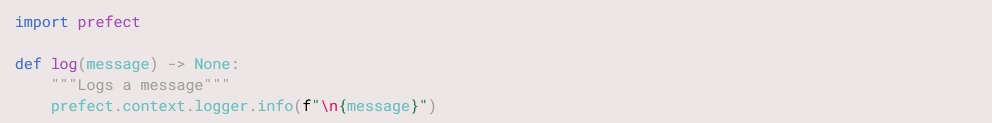
\includegraphics[width=\linewidth]{figs/2_7.png}
				\end{center}
			\end{block}
		\end{itemize}
	\end{frame}
	
	% Slide 23
	\begin{frame}{Desenvolvendo o Primeiro Flow}
		\textbf{Criando Funções Auxiliares}
		\begin{itemize}
			\item A função ``log'' recebe uma mensagem e a imprime no console.
			\item Ela faz isso através do objeto ``prefect.context.logger'', que é um objeto que contém o logger do Prefect.
			\item Esse logger é um objeto que está dentro do ``prefect.context'', esse que contém informações sobre o Flow e a execução atual, como por exemplo, o nome do Flow e o ID da execução atual.
			\item Por isso, é importante que essa função seja chamada dentro de um Flow, pois ela depende do objeto ``prefect.context'' para funcionar.
		\end{itemize}
	\end{frame}
	
	% Slide 24
	\begin{frame}{Desenvolvendo o Primeiro Flow}
		\textbf{Criando \textit{Tasks}}
		\begin{itemize}
			\item Aqui é onde serão criadas as funções que implementam os passos da pipeline.
			\item Essas funções serão chamadas de tasks.
			\item Então, abrindo o arquivo tasks.py, cria-se as seguintes funções:
		\end{itemize}
	\end{frame}
	
	% Slide 25
	\begin{frame}{Desenvolvendo o Primeiro Flow}
		\textbf{Criando \textit{Tasks}}
		\begin{block}{tasks.py (parte I)}
			\begin{center}
				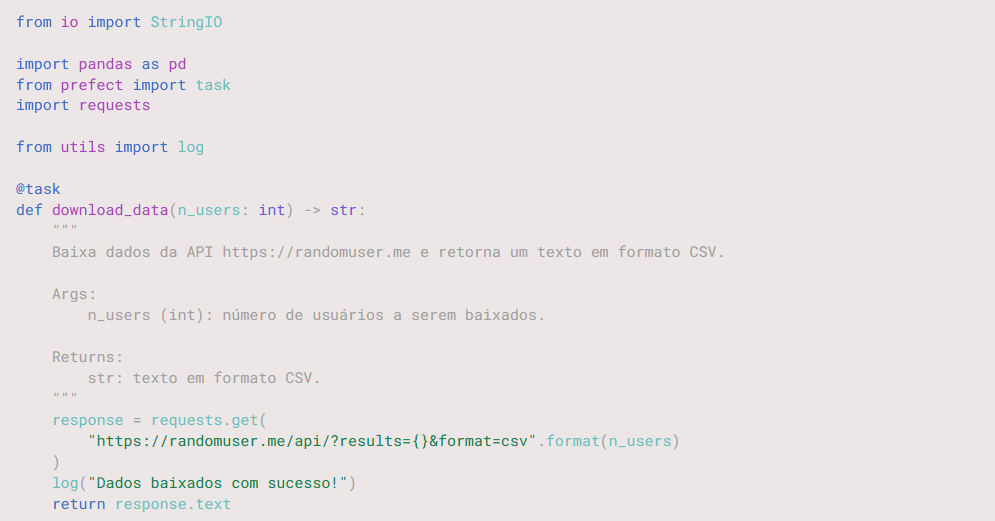
\includegraphics[width=\linewidth]{figs/2_8.png}
			\end{center}
		\end{block}
	\end{frame}
	
	% Slide 26
	\begin{frame}{Desenvolvendo o Primeiro Flow}
		\textbf{Criando \textit{Tasks}}
		\begin{block}{tasks.py (parte II)}
			\begin{center}
				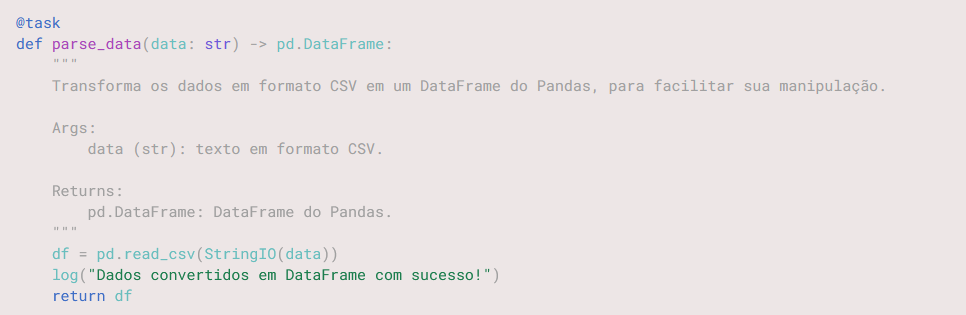
\includegraphics[width=\linewidth]{figs/2_9.png}
			\end{center}
		\end{block}
	\end{frame}
	
	% Slide 27
	\begin{frame}{Desenvolvendo o Primeiro Flow}
		\textbf{Criando \textit{Tasks}}
		\begin{block}{tasks.py (parte III)}
			\begin{center}
				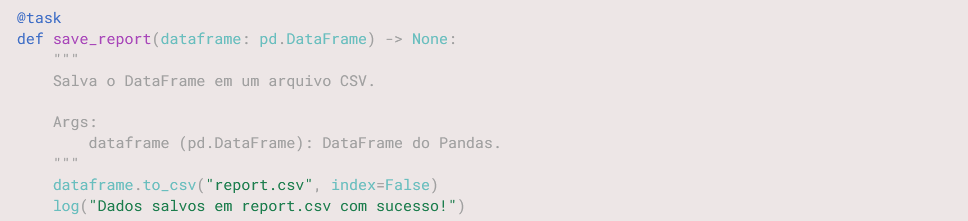
\includegraphics[width=\linewidth]{figs/2_10.png}
			\end{center}
		\end{block}
		\begin{itemize}
			\item Vale ressaltar que as funções são decoradas com o ``@task'', que é um decorator do Prefect.
			\item Esse decorator é necessário para que o Prefect reconheça as funções como tasks.
		\end{itemize}
	\end{frame}
	
	% Slide 28
	\begin{frame}{Desenvolvendo o Primeiro Flow}
		\textbf{Definindo um Flow}
		\begin{itemize}
			\item Agora, vamos criar o Flow propriamente dito.
			\item Aqui vamos definir como as tasks interagem entre si e os parâmetros que elas recebem. 
			\item Para isso, abra o arquivo flows.py e crie a seguinte função:
		\end{itemize}
		\begin{block}{flows.py}
			\begin{center}
				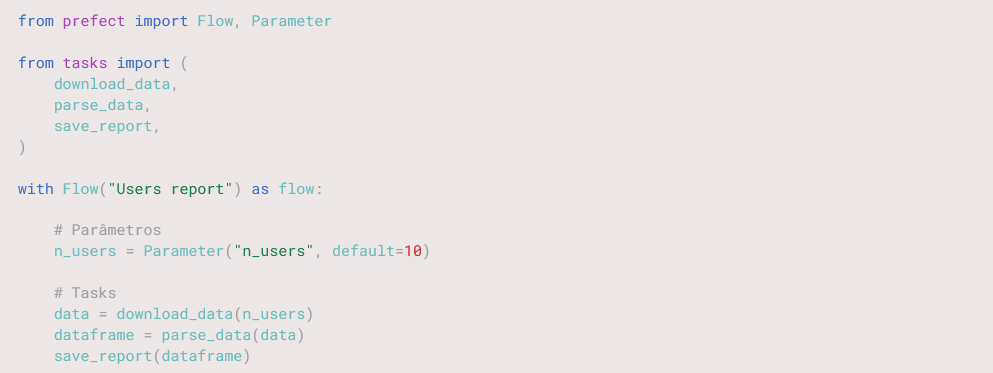
\includegraphics[width=\linewidth]{figs/2_11.png}
			\end{center}
		\end{block}
	\end{frame}
	
	% Slide 30
	\begin{frame}{Desenvolvendo o Primeiro Flow}
		\textbf{Definindo um Flow}
		\begin{itemize}
			\item Foi criado um Flow chamado ``Users report'' com o seguinte parâmetro:
			\begin{itemize}
				\item ``n\_users'': número de usuários a serem baixados.
			\end{itemize}
			\item Observe que foi configurado um valor padrão para esse parâmetro, que é 10.
			\item Isso significa que, caso o parâmetro não seja passado na hora de executar o Flow, ele será executado com o valor padrão.
		\end{itemize}
	\end{frame}
	
	% Slide 31
	\begin{frame}{Desenvolvendo o Primeiro Flow}
		\textbf{Definindo um Flow}
		\begin{itemize}
			\item Além disso, foram inseridas as três tasks criadas anteriormente.
			\item Observe que a task ``download\_data'' recebe o parâmetro ``n\_users'' como argumento.
			\item Isso significa que, quando a task for executada, ela receberá o valor do parâmetro ``n\_users'' como argumento.
			\item Depois disso, a task ``parse\_data'' recebe o retorno da task ``download\_data'' como argumento, fazendo com que o dado baixado seja passado a ela, para converter em um DataFrame.
			\item Por fim, a task ``save\_report'' recebe o retorno da task ``parse\_data'' como argumento, fazendo com que o DataFrame seja salvo em um arquivo CSV.
		\end{itemize}
	\end{frame}
	
	% Slide 32
	\begin{frame}{Desenvolvendo o Primeiro Flow}
		\textbf{Executando}
		\begin{itemize}
			\item Para facilitar a execução, cria-se um arquivo run.py com o seguinte código nele:
			\begin{block}{run.py}
				\begin{center}
					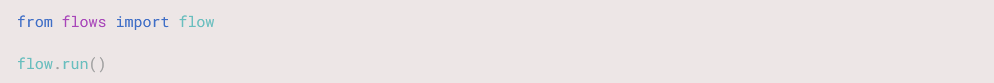
\includegraphics[width=\linewidth]{figs/2_12.png}
				\end{center}
			\end{block}
			\item Depois, pode-se executar o Flow com o seguinte comando:
			\begin{block}{cmd.exe}
				python3 run.py
			\end{block}
		\end{itemize}
	\end{frame}
	
	% Slide 33
	\begin{frame}{Desenvolvendo o Primeiro Flow}
		\textbf{Executando}
		\begin{itemize}
			\item A saída terá o seguinte formato:
			\begin{block}{}
				\begin{center}
					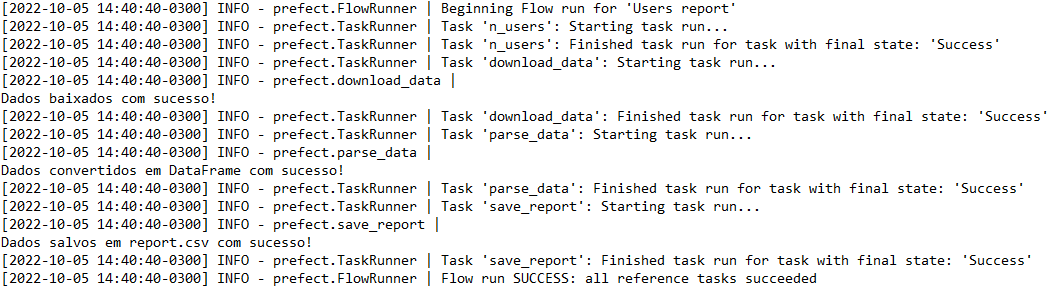
\includegraphics[width=\linewidth]{figs/2_13.png}
				\end{center}
			\end{block}
		\end{itemize}
	\end{frame}
	
	% Slide 34
	\begin{frame}{Desenvolvendo o Primeiro Flow}
		\textbf{Executando}
		\begin{itemize}
			\item Observe que um arquivo chamado ``report.csv'' foi criado.
			\item Esse arquivo contém os dados baixados e convertidos em um DataFrame.
			\item Observe também que as mensagens de log foram impressas na saída.
			\item Isso acontece porque, como vimos anteriormente, as funções ``log'' são decoradas com o ``@task'', que é um decorator do Prefect.
			\item Isso faz com que o Prefect reconheça as funções como tasks e, por isso, as mensagens de log são impressas na saída.
		\end{itemize}
	\end{frame}
	
\section{Referências}
	% Slide 19
	\begin{frame}{Referências}
		\begin{itemize}
			\item https://www.prefect.io - Informações gerais sobre a missão da empresa, recursos da ferramenta, Prefect Cloud e Prefect OSS.
			\item https://docs.prefect.io - Informações sobre a arquitetura, componentes (Flow, Task, Agent, Deployment), diferenças entre Prefect 1.x e 2.x, entre outras.
			\item https://medium.com/the-prefect-blog/why-not-airflow-4cfa423299c4 - Comparação direta com Airflow e descrição dos problemas enfrentados com DAGs estáticos.
			\item https://docs.dados.rio/guia-desenvolvedores/pipelines - Desenvolvimento de pipelines local.
			\item https://discourse.prefect.io - Comunidade Prefect no Discourse
		\end{itemize}
	\end{frame}
\end{document}
